\documentclass[dvisvgm]{standalone}
\usepackage{tikz}
\usepackage{tikz-3dplot}
\usepackage{pgfplots}
\pgfplotsset{compat=1.18}

\begin{document}

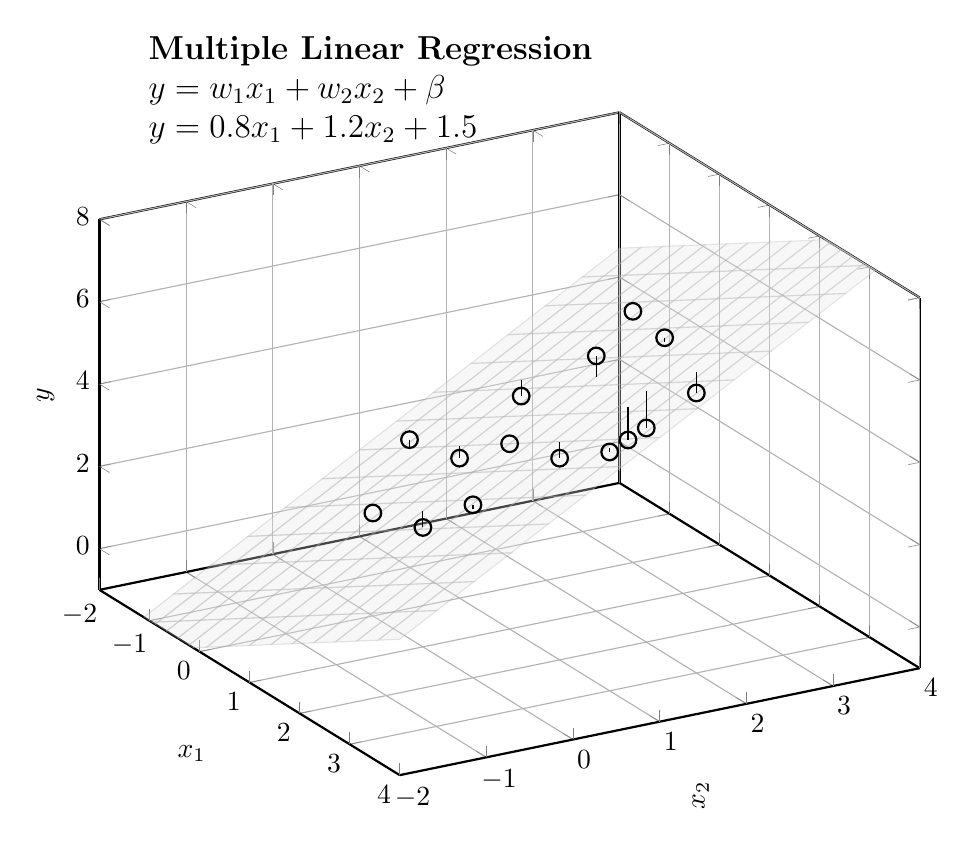
\begin{tikzpicture}
\begin{axis}[
    view={60}{30},
    width=12cm,
    height=10cm,
    xlabel={$x_1$},
    ylabel={$x_2$},
    zlabel={$y$},
    xlabel style={anchor=north east},
    ylabel style={anchor=north west},
    zlabel style={anchor=south},
    grid=major,
    axis lines=box,
    axis line style={black, thick},
    grid style={black!30, thin},
    axis background/.style={fill=white},
    xmin=-2, xmax=4,
    ymin=-2, ymax=4,
    zmin=-1, zmax=8,
    xtick={-2,-1,0,1,2,3,4},
    ytick={-2,-1,0,1,2,3,4},
    ztick={0,2,4,6,8},
]

% Regression plane: y = 0.8*x1 + 1.2*x2 + 1.5
\addplot3[
    surf,
    domain=-2:4,
    domain y=-2:4,
    samples=15,
    samples y=15,
    opacity=0.3,
    fill=black!10,
    draw=black,
    mesh/interior colormap name=,
    colormap={bw}{gray(0cm)=(0.8); gray(1cm)=(0.9)},
] {0.8*x + 1.2*y + 1.5};

% All data points as circles
\addplot3[
    only marks,
    mark=o,
    mark size=3pt,
    color=black,
    mark options={thick},
] coordinates {
    (1, 2, 5.2)    % Expected: 4.7, Actual: 5.2
    (3, 1, 4.8)    % Expected: 4.9, Actual: 4.8  
    (0, 3, 5.1)    % Expected: 5.1, Actual: 5.1
    (2, 0, 3.2)    % Expected: 3.1, Actual: 3.2
    (-1, 1, 2.1)   % Expected: 1.9, Actual: 2.1
    (1.5, 2.5, 5.8) % Expected: 5.7, Actual: 5.8
    (2, 2, 4.2)    % Expected: 5.1, Actual: 4.2
    (0, 1, 2.4)    % Expected: 2.7, Actual: 2.4
    (3, 2, 5.8)    % Expected: 6.3, Actual: 5.8
    (-0.5, 2, 3.1) % Expected: 3.5, Actual: 3.1
    (1, 0, 1.9)    % Expected: 2.3, Actual: 1.9
    (2.5, 1.5, 4.5) % Expected: 5.3, Actual: 4.5
    (0, 0, 1.5)    % Expected: 1.5, Actual: 1.5
    (1, 1, 3.5)    % Expected: 3.5, Actual: 3.5
    (2, 1, 3.9)    % Expected: 4.3, Actual: 3.9
};

% Vertical lines from points to regression plane (residuals)
\addplot3[black, thin, no marks] coordinates {(1, 2, 5.2) (1, 2, 4.7)};
\addplot3[black, thin, no marks] coordinates {(3, 1, 4.8) (3, 1, 4.9)};
\addplot3[black, thin, no marks] coordinates {(0, 3, 5.1) (0, 3, 5.1)};
\addplot3[black, thin, no marks] coordinates {(2, 0, 3.2) (2, 0, 3.1)};
\addplot3[black, thin, no marks] coordinates {(-1, 1, 2.1) (-1, 1, 1.9)};
\addplot3[black, thin, no marks] coordinates {(1.5, 2.5, 5.8) (1.5, 2.5, 5.7)};
\addplot3[black, thin, no marks] coordinates {(2, 2, 4.2) (2, 2, 5.1)};
\addplot3[black, thin, no marks] coordinates {(0, 1, 2.4) (0, 1, 2.7)};
\addplot3[black, thin, no marks] coordinates {(3, 2, 5.8) (3, 2, 6.3)};
\addplot3[black, thin, no marks] coordinates {(-0.5, 2, 3.1) (-0.5, 2, 3.5)};
\addplot3[black, thin, no marks] coordinates {(1, 0, 1.9) (1, 0, 2.3)};
\addplot3[black, thin, no marks] coordinates {(2.5, 1.5, 4.5) (2.5, 1.5, 5.3)};
\addplot3[black, thin, no marks] coordinates {(0, 0, 1.5) (0, 0, 1.5)};
\addplot3[black, thin, no marks] coordinates {(1, 1, 3.5) (1, 1, 3.5)};
\addplot3[black, thin, no marks] coordinates {(2, 1, 3.9) (2, 1, 4.3)};

\end{axis}

% Add equation
\node[anchor=north west, align=left, font=\large] at (0.5, 9.5) {
    \textbf{Multiple Linear Regression} \\
    $y = w_1 x_1 + w_2 x_2 + \beta$ \\
    $y = 0.8 x_1 + 1.2 x_2 + 1.5$
};

\end{tikzpicture}

\end{document}
